\chapter{ユーザ情報の偏在化}\label{chap:implementation_2}

ここでは、そこにいる名無しさんを補助する目的で作られたユーザ管理システムについて述べる。

\newpage

\section{概要}

\subsection{本補助システムの目的}

そこにいる名無しさんのシステムでは、近くにユーザ数が確保できない限り、
アクティビティの内容が活性化しないという問題があった。

近年では人々が持ち歩くモバイルデバイスは、スマートフォンだけに留まらず、様々なデバイスを持ち歩くようになってきている。
そのなかでも、Bluetoothモジュールは大抵のモバイルデバイスに付属しており、
Bluetooth近接検出では一人の人間に対して復数のデバイスを検出することもままある。

本システムは、本論文の実装物であるそこにいる名無しさんの効果を高めるため、
ユーザが持つモバイルデバイスとは別に、スレイヴとして別端末も同じユーザとみなす効果をもたらすための
アプリケーションである。

\begin{figure}[b]
  \begin{center}
    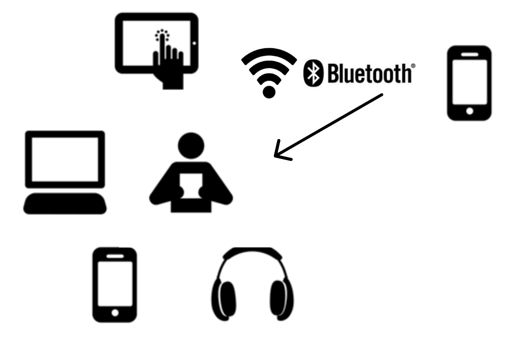
\includegraphics[width=0.5\linewidth]{img/sub.eps}
  \end{center}
  \caption{人の持つBluetoothモジュール}
  \label{fig:sub}
\end{figure}

\newpage

\section{設計}

\subsection{デバイスの検出とユーザが結びつく確実性}

ここまでは、ユーザと紐付いたデバイスが検出されたならば、そこにユーザが居るという前提に立って述べてきた。
しかしユーザが持っているデバイスは一つとは限らず、検出されるのが紐付いたデバイスであるとは限らない。
例えば分厚い鞄に入ったデバイスは、電波状況のために検出から逸れることもままある。
また、Bluetoothを何らかの要因で
その場合に予備としてユーザと紐付いたデバイスがあれば、周囲のアプリケーションからは同じ効果が得られる。


\subsection{同じユーザであると認められるデバイス}

Bluetoothモジュールを持っており、同じユーザであると認めることのできるデバイスには、
以下が考えられる。

\begin{itemize}

\item アプリケーションがインストールされたモバイルデバイス

\item タブレットなど、サブ用途であるモバイルデバイス

\item モバイル用途のコンピュータ

\item Bluetoothモジュールを持ったヘッドホン(イヤホン)

\end{itemize}

\subsection{認められるデバイスの数}

以上のように個人でも復数のBluetoothモジュールを持つデバイスを持つことが考えられるため、
本補助システムでは、最大4つまでのデバイスを同じユーザとして登録することを認めることにした。


\newpage

\section{実装}

\subsection{システム構成}

本システムは、そこにいる名無しさんと同じく、Androidアプリケーション、APIサーバ、データベースの3つで構成されている。

AndroidアプリケーションはJava、APIサーバはNode.js0.10、以降のシステムはそこにいる名無しさんと共有している。

\subsection{APIインターフェイス}

\begin{description}

  \item{adduser}

adduserからは、既に登録されたMACアドレスとユーザID、新たに追加するMACアドレスを受け付ける。
サーバは、既に登録されたMACアドレスからユーザ情報をデータベースから取り寄せ、
新たに追加するMACアドレスをスレイヴとして登録する。

\end{description}

\subsection{アプリケーション}

アプリケーションはそこにいる名無しさんと同じくBluetooth2.1プロトコルの検出機能を利用し、
周囲のデバイスを検出する。このとき、検出対象になるのはアプリケーションが入っているモバイルデバイスと
既にペアリングされているデバイスのみである。

アプリケーションはペアリングされているデバイスをユーザのスレイヴデバイスとみなし、
APIサーバに自らのMACアドレスと、スレイヴとみなすデバイスのMACアドレスを送信する。

これにより、以降はそこにいる名無しさん側でも、スレイヴデバイスをユーザの持つモバイルデバイスと見なすようになる。
